\documentclass{article}
\title{Optimizing a Path Tracer}
\author{Kristoffer Lundgren}

\usepackage{listings}
\usepackage{color}
\usepackage{xcolor}
\usepackage{graphicx}

\lstset{%
    language=c++,
    backgroundcolor=\color{black!5}, 
    basicstyle=\footnotesize
}
\definecolor{dkgreen}{rgb}{0,0.6,0}
\definecolor{gray}{rgb}{0.5,0.5,0.5}
\definecolor{mauve}{rgb}{0.58,0,0.82}

\lstset{frame=tb,
  language=Java,
  aboveskip=3mm,
  belowskip=3mm,
  showstringspaces=false,
  columns=flexible,
  basicstyle={\small\ttfamily},
  numbers=none,
  numberstyle=\tiny\color{gray},
  keywordstyle=\color{blue},
  commentstyle=\color{dkgreen},
  stringstyle=\color{mauve},
  breaklines=true,
  breakatwhitespace=true,
  tabsize=3
}

\begin{document}

\maketitle
\pagenumbering{gobble}
\newpage
\pagenumbering{arabic}

\section{Valgrind Static Code Analysis}
    \begin{figure}[!htb]
        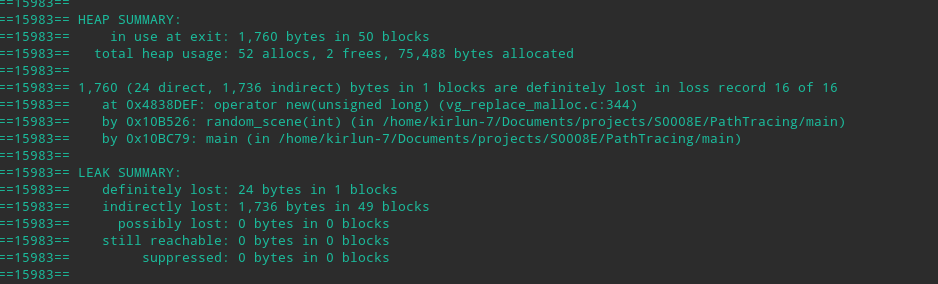
\includegraphics[width=\linewidth]{first_analysis.png}
        \caption{First Analysis}
        \label{fig:a1}
    \end{figure}
    The first Valgrind analysis revealed a lot of memory leaks but that was to be expected
    I had made no effort to prevent memory leaks. I then added a deconstructor in the hitableList class which in turn loops through all its contents and calls their destructors.
    \begin{figure}[!htb]
        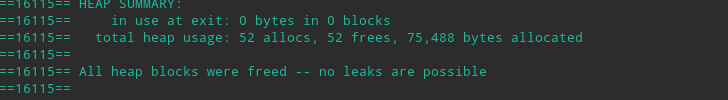
\includegraphics[width=\linewidth]{after_deletes.png}
        \caption{After Adding deconstructors}
        \label{fig:a2}
    \end{figure}
\newpage
\section{Optimizing}
    In order to optimize my path tracer i implemented simple multithreading since that provides the best performance impact. The threads each run a function that calculates a pixel, when a pixel is
    complete it calls a function to ask for another pixel.

    \begin{lstlisting}
    void calcPixel(int ns, hitable * world, int nx, int ny, camera cam)
    {
        while(1)
        {
            pixel* currentPixel = cont.getPixel();
            if(currentPixel == nullptr)
                break;
            Vector4D col(0,0,0,1);
            for (int i = 0; i < ns; ++i)
            {
                float u = float(currentPixel->x + xorShift())/float(nx);
                float v = float(currentPixel->y + xorShift())/float(ny);
                ray r = cam.getRay(u, v);
                Vector4D p = r.pointAtParameter(2.0);
                col = col + color(r, world, 0);
    
            }
            col = col / float(ns);
            col = Vector4D(sqrt(col[0]), sqrt(col[1]), sqrt(col[2]), 1);
            currentPixel->r = int(255.99*col[0]);
            currentPixel->g = int(255.99*col[1]);
            currentPixel->b = int(255.99*col[2]);
        }
    }
    \end{lstlisting}
    This code snippet starts six threads that all run the function seen above.
    \begin{lstlisting}
    std::thread threads[6];
    for (int m = 0; m < 6; ++m)
    {
        threads[m] = std::thread(calcPixel, ns, world, nx, ny, cam);
    }
    for (int j = 0; j < 6; ++j)
    {
        threads[j].join();
    }
    \end{lstlisting}

\end{document}
